\section{问题二：跨维度数据融合与广义标度律}
\label{sec:problem2}

\subsection{建模思路与可检验假设}

附件中没有同时改变 $N,D,Q,\boldsymbol p$ 的联合实验：B1 只改变 $(N,D)$；B7 在固定的 $(N,D)$ 网格上改变质量；附件 A 只改变配比。因此广义标度律必须具有\textbf{可分结构}——每一项只由一类数据识别——再用可检验的假设把它们统一起来。我们提出如下三条假设，并在后文逐一检验：

\begin{assumption}[参数—数据可分]\label{hyp:sep}
在固定质量与配比下，Loss 为不可约项、参数项、数据项之和，即 $L=E+An^{-\alpha}+Bd^{-\beta}$，参数与数据之间无额外交互。（检验：\S\ref{sec:p2_classic}，与含交互项模型对比。）
\end{assumption}

\begin{assumption}[质量加性惩罚且可退化]\label{hyp:quality}
数据质量偏离理想状态时，在经典项之上产生附加损失 $\Delta_Q(Q)\ge0$，且 $\Delta_Q(1)=0$，即 $Q=1$ 时广义标度律严格退化为经典形式。（检验：\S\ref{sec:p2_quality}，四种质量函数形式的成块交叉验证。）
\end{assumption}

\begin{assumption}[配比效应尺度不变]\label{hyp:mix}
领域配比按比例缩放\textbf{可约损失} $L-E$，缩放因子 $\exp[\theta R(\boldsymbol p)]$ 中的系数 $\theta$ 不随模型规模变化。这是连接附件 A（配比实验）与附件 B（规模实验）的桥梁：两套实验的绝对 Loss 不可比，但“可约损失被配比改变了百分之几”是无量纲、可迁移的。（检验：\S\ref{sec:p2_mixture}，附件 A 的 1M、60M、1B 三个规模。）
\end{assumption}

数据的使用分工见表~\ref{tab:p2_data}。B6--B8、B10 为半合成或估算数据，本文只将其用于补充分析与边界检验，不作为直接实验观测。

\begin{table}[htbp]
\centering
\small
\caption{问题二的数据分工}
\label{tab:p2_data}
\begin{tabular}{p{0.12\linewidth}p{0.36\linewidth}p{0.42\linewidth}}
\toprule
数据 & 性质 & 用途 \\
\midrule
B1 & 真实训练轨迹，8 个参数规模、1176 个检查点 & 经典标度律主拟合与留一规模验证 \\
B2 & 半合成族外轨迹 & 冻结参数后的族外验证 \\
B4 / B5 & 跨模型族记录 / 文献数据 & 跨族与文献验证 \\
B6 / B7 & 质量分块实验（B6 为 B7 子集），$45$ 个 $(N,D)$ 单元 × 10 档质量 & B7 拟合质量项，B6 做一致性核对 \\
B8 & 扩展质量网格（半合成） & 压力测试与外推边界 \\
B9 / B10 & 百亿参数以上模型信息 / 估算 Loss & 大规模外推讨论 \\
A4--A11 & 问题一的配比实验与检验集 & 配比效应系数 $\theta$ 的标定与尺度不变性检验 \\
\bottomrule
\end{tabular}
\end{table}

\subsection{经典标度律}
\label{sec:p2_classic}

\subsubsection{候选模型与估计方法}

记 $n=N/10^9$，$d=D/10^9$。比较三种候选结构：
\begin{align}
M_0:&\quad L=E+An^{-\alpha}+Bd^{-\beta}, \label{eq:p2_m0}\\
M_C:&\quad L=E_C+K_C(6nd)^{-\zeta}, \label{eq:p2_mc}\\
M_{ND}:&\quad L=E+An^{-\alpha}+Bd^{-\beta}+G(nd)^{-\xi}. \label{eq:p2_mnd}
\end{align}
$M_0$ 即 Chinchilla 形式\cite{hoffmann2022compute}；$M_C$ 假设 Loss 只依赖总算力\cite{kaplan2020scaling}；$M_{ND}$ 在 $M_0$ 上加入参数—数据交互项，用于检验假设~\ref{hyp:sep}。所有系数与指数约束为正（对数参数化 $\theta=e^{\eta}$），保证 Loss 随资源单调不增。以模型规模为聚类单元赋等权，用 Huber 稳健非线性最小二乘估计，并以拉丁超立方采样的 50 个起点避免局部极小。模型评价采用\textbf{留一参数规模}交叉验证：每次留出一个规模的整条轨迹，这比随机留点更严格地检验了对新规模的外推能力。

\subsubsection{结果}

\begin{table}[htbp]
\centering
\small
\caption{经典标度律候选模型的留一参数规模验证}
\label{tab:p2_classic}
\begin{tabular}{lccc}
\toprule
模型 & 留一规模 RMSE & 归一化 RMSE & 参数个数 \\
\midrule
$M_0$（可分幂律） & $\mathbf{1.47\times10^{-4}}$ & $\mathbf{3.74\times10^{-4}}$ & 5 \\
$M_C$（总算力幂律） & $8.49\times10^{-2}$ & $2.16\times10^{-1}$ & 3 \\
$M_{ND}$（含交互项） & $1.48\times10^{-4}$ & $3.76\times10^{-4}$ & 7 \\
\bottomrule
\end{tabular}
\end{table}

由表~\ref{tab:p2_classic}：（1）$M_C$ 的误差比 $M_0$ 大近 600 倍，说明相同算力下 $N$ 与 $D$ 的分配方式对 Loss 有决定性影响，这正是问题三资源配置有意义的前提；（2）$M_{ND}$ 增加两个参数后误差没有下降，交互项不提供额外解释力，\textbf{假设~\ref{hyp:sep} 成立}。按一倍标准误原则选择 $M_0$，500 次聚类 bootstrap 给出的参数及 95\% 区间为
\begin{equation}
\begin{aligned}
E&=1.6898\ [1.6897,1.6899], & A&=0.3540\ [0.3539,0.3541], & \alpha&=0.3400\ [0.3399,0.3401],\\
& & B&=1.2403\ [1.2402,1.2404], & \beta&=0.2799\ [0.2798,0.2799].
\end{aligned}
\label{eq:p2_classic_est}
\end{equation}

图~\ref{fig:p2_classic}(b) 给出一个更直观的检验：若 $M_0$ 正确，则扣除参数项后的“剩余损失” $L-E-An^{-\alpha}$ 应只依赖 $d$。8 个规模、共 1176 个检查点在双对数坐标下\textbf{坍缩到同一条斜率为 $-\beta$ 的直线}上，各规模残差 RMSE 均在 $(1.0\sim2.1)\times10^{-4}$ 之间且中位数接近 0。剔除 $D<2\mathrm{B}$ 的 32 个早期检查点后重新拟合，参数的最大相对变化仅 $0.053\%$。

\begin{figure}[htbp]
\centering
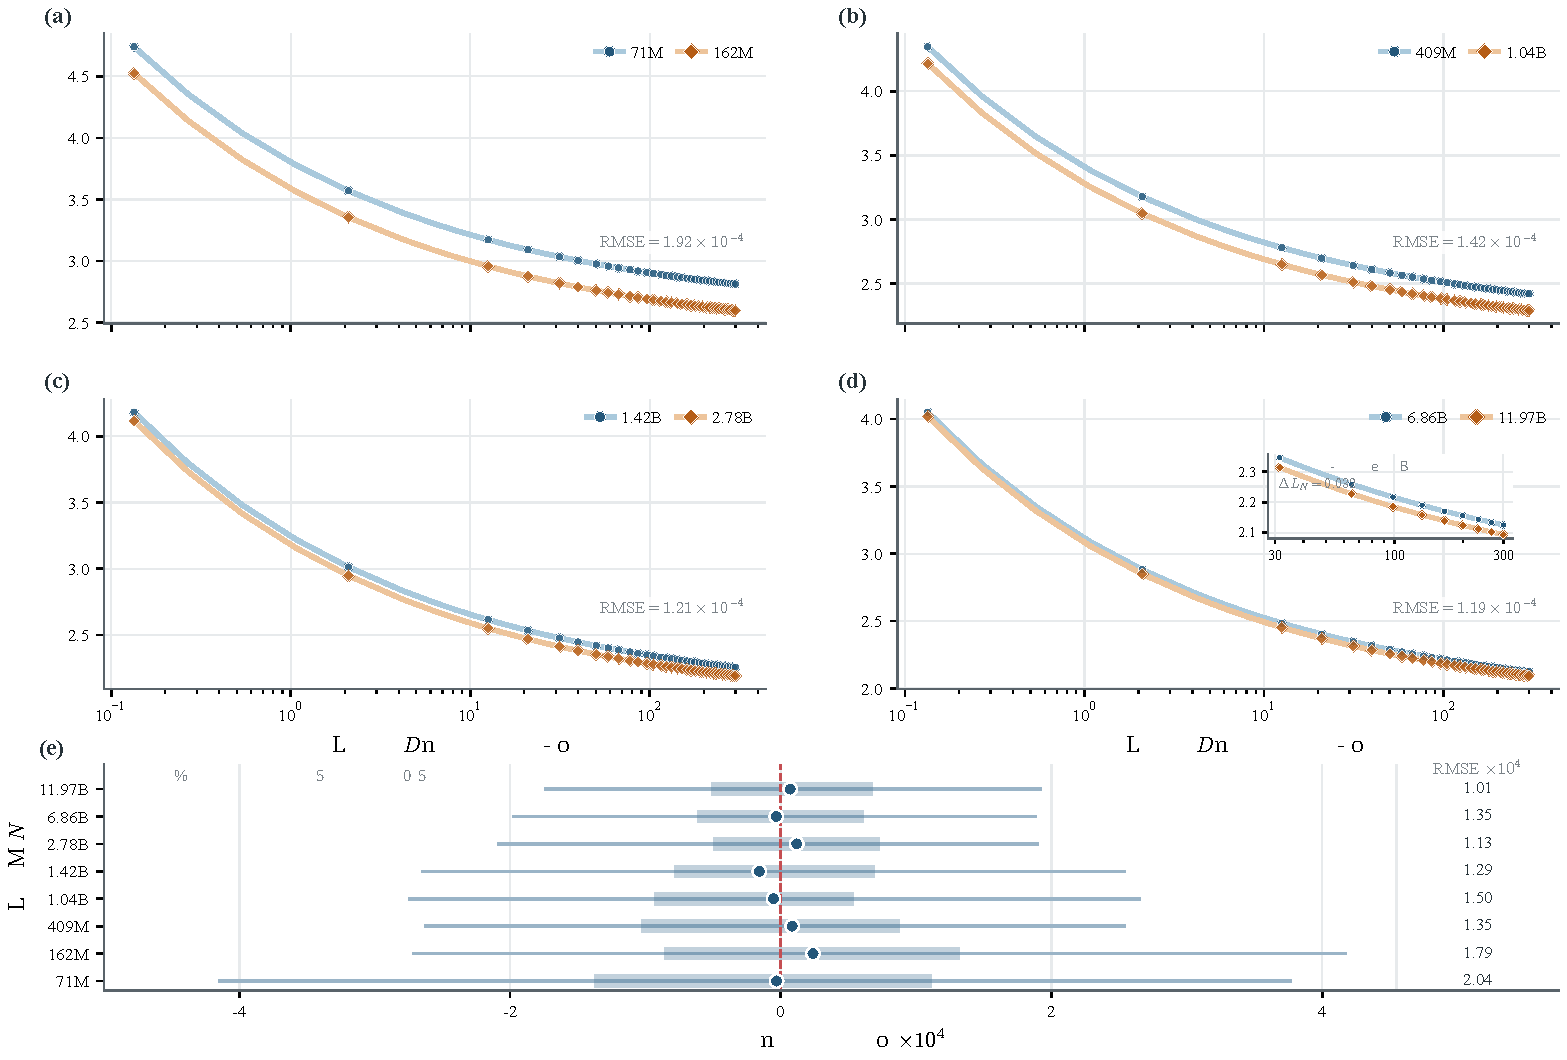
\includegraphics[width=\linewidth]{images/no2/P2R_F01_经典标度律拟合与数据坍缩.pdf}
\caption{经典标度律：B1 八个规模的拟合（a）、数据坍缩检验（b）与各规模残差（c）}
\label{fig:p2_classic}
\end{figure}

由 $M_0$ 可以直接推出计算最优配置的标度指数：在 $C=6ND$ 约束下最小化 $L$ 得 $N^*\propto C^{\beta/(\alpha+\beta)}=C^{0.452}$，$D^*\propto C^{\alpha/(\alpha+\beta)}=C^{0.548}$，与 Chinchilla 研究报告的 $0.46/0.54$ 高度一致\cite{hoffmann2022compute,besiroglu2024chinchilla}。这为本文标度律的外部有效性提供了文献层面的佐证。

\subsection{质量修正项}
\label{sec:p2_quality}

\subsubsection{候选形式}

在固定 B1 经典参数的前提下，用 B7 质量网格估计质量惩罚项 $\Delta_Q$。设计四种满足 $\Delta_Q(1)=0$ 的候选形式，分别对应四种关于“质量如何起作用”的机制假说：
\begin{align}
\text{GQ1（有效样本量）}:&\quad \Delta_Q=Bd^{-\beta}\left(Q^{-\gamma}-1\right), \label{eq:gq1}\\
\text{GQ2（加性惩罚）}:&\quad \Delta_Q=c_Q(1-Q)^{\nu_Q}, \label{eq:gq2}\\
\text{GQ3（指数变化）}:&\quad \Delta_Q=Bd^{-\beta}\left[e^{b_Q(1-Q)}d^{-\beta_1(1-Q)}-1\right], \label{eq:gq3}\\
\text{GQ4（双通道）}:&\quad \Delta_Q=An^{-\alpha}\left(Q^{-\alpha\gamma_N}-1\right)+Bd^{-\beta}\left(Q^{-\beta\gamma_D}-1\right). \label{eq:gq4}
\end{align}
GQ1 把低质量数据视为“打了折扣的有效 Token”（$D_{\mathrm{eff}}=Q^{\gamma/\beta}D$），与数据受限标度律的思想一致\cite{muennighoff2023dataconstrained}；GQ2 认为低质量引入一个与规模无关的额外损失；GQ3 允许质量改变数据项的指数；GQ4 让质量同时折扣参数与数据的有效规模。

\subsubsection{成块交叉验证选择}

为避免信息泄漏，验证按\textbf{参数规模、数据规模、质量水平、$(N,D)$ 单元}四种方式成块留出（共 69 个留出块），四类切分等权，且验证折中不提供该单元 $Q=1$ 的基线 Loss。结果见图~\ref{fig:p2_quality}。

\begin{figure}[htbp]
\centering
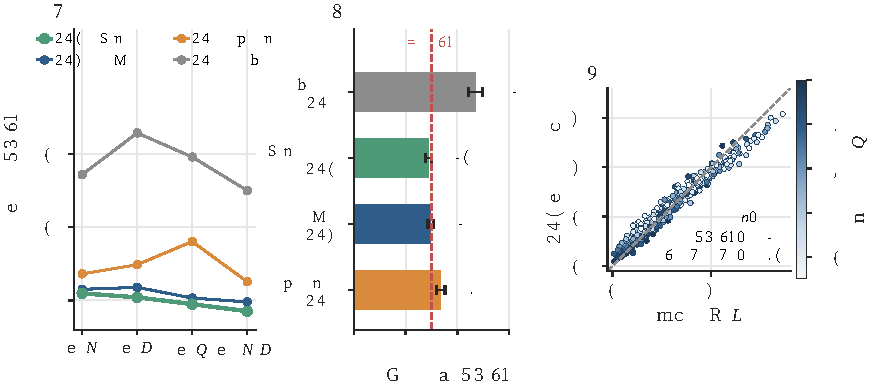
\includegraphics[width=\linewidth]{images/no2/P2R_F02_质量模型成块交叉验证选择.pdf}
\caption{质量修正项的成块交叉验证：各切分误差（a）、等权 RMSE（b）与 GQ2 留单元预测（c）}
\label{fig:p2_quality}
\end{figure}

GQ2 在全部四种切分下误差均最低（nRMSE $0.143$--$0.155$，GQ1 为 $0.225$--$0.264$），等权 RMSE 为 $0.0720$，比 GQ1 低 $38.7\%$；在 69 个留出块中 GQ2 最优的有 41 个。GQ3 与 GQ2 参数个数相同，其等权 RMSE（$0.0744$）落在一倍标准误阈值（$0.0747$）之内、差异不显著；GQ2 误差最低且形式最简、可解释性最好，故选择 GQ2。留 $(N,D)$ 单元验证中，GQ2 预测与观测的 Spearman 系数达 $0.982$，只在高 Loss 尾部略有低估。500 次单元聚类 bootstrap 给出
\begin{equation}
c_Q=0.3620\ [0.3327,0.3923],\qquad \nu_Q=0.990\ [0.918,1.068].
\label{eq:p2_quality_est}
\end{equation}
$\nu_Q$ 的区间包含 1，说明在 B7 支持域内\textbf{质量惩罚近似与质量缺口 $1-Q$ 成正比}：质量每提高 $0.1$，Loss 约降低 $0.036$（bootstrap 95\% 区间 $[0.033,0.039]$），且这一收益不随模型规模衰减——这正是后文“规模越大、质量越值钱”的根源。

GQ2 优于 GQ1 的事实本身也有含义：若低质量只是“稀释了有效 Token”，其损害应随 $D$ 增大而减小（GQ1）；数据却支持一个与 $D$ 无关的惩罚。这表明\textbf{低质量数据带来的损失无法靠堆砌数据量弥补}，与数据剪枝研究中“质量可突破幂律”的发现相呼应\cite{sorscher2022beyond}。

\subsubsection{与问题一质量尺度的对接}

问题一的质量评分 $Q_A$ 与 B7 的质量字段来自不同体系。以问题一参考配比对应的质量 $Q_{\mathrm{ref}}=\boldsymbol p_{\mathrm{ref}}^{\mathsf T}\boldsymbol q=0.5390$ 为公共锚点，令
\begin{equation}
Q_{\mathrm{eff}}=\operatorname{clip}\!\left[Q_{\mathrm{ref}}+s_Q(Q_A-Q_{\mathrm{ref}}),\ \varepsilon,\ 1\right],\qquad s_Q\in\{0.5,\ 1,\ 1.5\},
\label{eq:p2_qmap}
\end{equation}
主情景取 $s_Q=1$（两套质量尺度等距对应），$s_Q=0.5,1.5$ 用于敏感性分析。这样，问题一的领域质量与配比通过基线质量 $Q_0(\boldsymbol p)=\boldsymbol p^{\mathsf T}\boldsymbol q$ 进入广义标度律。

\subsection{配比修正项与尺度不变性检验}
\label{sec:p2_mixture}

\subsubsection{标准化配比响应}

由问题一的 Scheff\'e--Ridge 响应面 $\widehat L_k(\boldsymbol p)$ 与综合目标 $J(\boldsymbol p)$（式~\eqref{eq:p1_J}），定义以参考配比为零点的标准化配比响应
\begin{equation}
R(\boldsymbol p)=\frac{J(\boldsymbol p)-J(\boldsymbol p_{\mathrm{ref}})}{\operatorname{IQR}_{\mathrm{A4}}\!\left[J\right]},\qquad R(\boldsymbol p_{\mathrm{ref}})=0,
\label{eq:p2_R}
\end{equation}
分母为 512 组训练配方上 $J$ 的四分位距。$R<0$ 表示配比优于参考配比；问题一的近优配比 $R(\boldsymbol p^\star)=-2.290$（bootstrap 95\% 区间 $[-3.568,\,0.113]$）。

\subsubsection{系数 $\theta$ 的标定}

在附件 A 的三个实测检验规模（1M、60M、1B）上，分别以 $R(\boldsymbol p)$ 为自变量、13 域平均 Loss 为因变量做稳健回归，得到截距 $\bar L(n)$（参考配比处的平均 Loss）与斜率 $s(n)=\partial L/\partial R$。若假设~\ref{hyp:mix} 成立，由 $L=E+(\bar L-E)e^{\theta R}$ 得 $\partial L/\partial R|_{R=0}=\theta(\bar L-E)$，于是
\begin{equation}
\theta(n)=\frac{s(n)}{\bar L(n)-E}.
\label{eq:p2_theta}
\end{equation}
各规模的估计见表~\ref{tab:p2_theta} 与图~\ref{fig:p2_mix}。

\begin{table}[htbp]
\centering
\small
\caption{配比效应的绝对强度 $s(n)$ 与相对强度 $\theta(n)$}
\label{tab:p2_theta}
\begin{tabular}{lccccccc}
\toprule
规模 & 配方数 & Spearman$(R,L)$ & $s(n)$ & $\bar L(n)$ & $\theta(n)$ & $\theta$（$E=1.5$） & $\theta$（$E=1.9$） \\
\midrule
1M & 256 & 0.813 & 0.2689 & 5.567 & 0.0693 & 0.0661 & 0.0733 \\
60M & 256 & 0.820 & 0.2386 & 4.152 & 0.0969 & 0.0900 & 0.1059 \\
1B & 64 & 0.734 & 0.0840 & 2.646 & 0.0878 & 0.0733 & 0.1125 \\
\midrule
\multicolumn{3}{l}{1B 相对 1M 的比值} & $0.312$ & — & $1.27$ & $1.11$ & $1.53$ \\
\bottomrule
\end{tabular}
\end{table}

\begin{figure}[htbp]
\centering
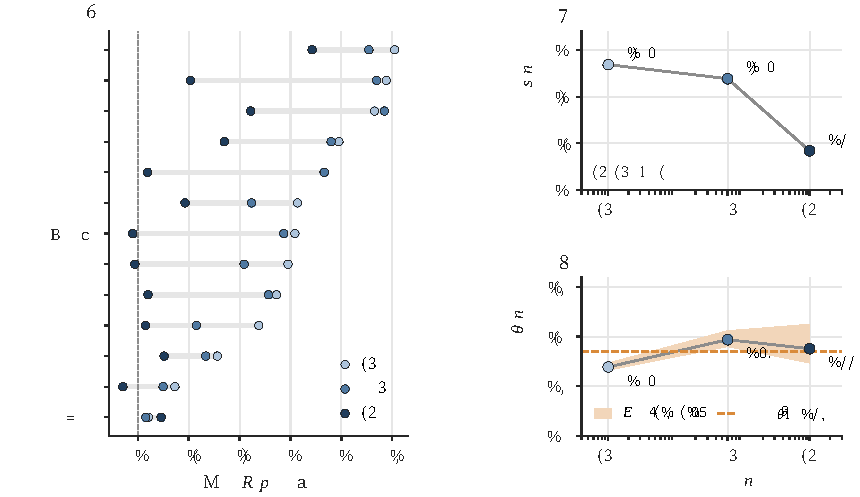
\includegraphics[width=\linewidth]{images/no2/P2R_F05_配比效应跨尺度迁移.pdf}
\caption{配比效应的跨规模迁移：各验证域斜率（a）、绝对强度 $s(n)$（b）与相对强度 $\theta(n)$（c）}
\label{fig:p2_mix}
\end{figure}

结果清楚地支持假设~\ref{hyp:mix}：规模从 1M 增至 1B（三个数量级），配比效应的\textbf{绝对}强度下降了 $69\%$（$0.269\to0.084$），但它占可约损失的\textbf{相对}比例 $\theta$ 始终稳定在 $0.07$--$0.10$，三个规模的变异系数仅 $0.17$，取 $E=1.5$ 时结论不变；取 $E=1.9$ 时 $\theta$ 随规模略有上升（1B 与 1M 之比为 $1.53$），但这一变化远小于绝对强度 $69\%$ 的降幅，且方向与“配比效应随规模消失”相反。这说明\textbf{配比改变的是“剩余可降低部分”的百分比，而非固定的 Loss 差值}——这也解释了问题一中 1B 上排序保持良好而绝对 $R^2$ 下降的现象，并与数据混合律中“Loss 对配比呈指数依赖”的经验形式一致\cite{ye2025datamixinglaws}。取三个规模的平均值
\begin{equation}
\theta=0.0847\qquad(\text{变异系数 } 0.17).
\label{eq:p2_theta_est}
\end{equation}

\subsection{广义标度律}

\subsubsection{模型形式}

综合式~\eqref{eq:p2_m0}、\eqref{eq:gq2}、\eqref{eq:p2_qmap}、\eqref{eq:p2_R} 与假设~\ref{hyp:mix}，本文提出的广义标度律为
\begin{equation}
\boxed{\;
L(N,D,Q,\boldsymbol p)=E+\Big[\,A n^{-\alpha}+B d^{-\beta}+c_Q\,(1-Q_{\mathrm{eff}})^{\nu_Q}\Big]\cdot \exp\!\big[\theta R(\boldsymbol p)\big]
\;}
\label{eq:p2_GSL}
\end{equation}
其中 $Q_{\mathrm{eff}}$ 由式~\eqref{eq:p2_qmap} 给出，基线质量 $Q_0(\boldsymbol p)=\boldsymbol p^{\mathsf T}\boldsymbol q$ 由问题一的领域质量与配比决定，质量处理可将其提升至 $Q_A\ge Q_0$。代入估计值：
\begin{equation}
L=1.6898+\Big[0.3540\,n^{-0.3400}+1.2403\,d^{-0.2799}+0.3620\,(1-Q_{\mathrm{eff}})^{0.9903}\Big]\,e^{\,0.0847\,R(\boldsymbol p)} .
\label{eq:p2_GSL_num}
\end{equation}

\subsubsection{模型性质}

\begin{theorem}[广义标度律的基本性质]\label{thm:gsl}
式~\eqref{eq:p2_GSL} 满足：
\begin{enumerate}
\item \textbf{退化性}：当 $Q_{\mathrm{eff}}=1$、$\boldsymbol p=\boldsymbol p_{\mathrm{ref}}$ 时，$L=E+An^{-\alpha}+Bd^{-\beta}$，严格退化为经典标度律；
\item \textbf{单调性}：$L$ 关于 $N$、$D$、$Q_{\mathrm{eff}}$ 严格递减，关于 $R(\boldsymbol p)$ 严格递增；
\item \textbf{物理下界}：对任意 $N,D,Q,\boldsymbol p$，恒有 $L>E$，即任何资源组合都不能突破不可约损失；
\item \textbf{配比可分性}：对任意固定的 $\boldsymbol p$，$\arg\min_{N,D,Q}L$ 与 $\boldsymbol p$ 无关。
\end{enumerate}
\end{theorem}

\noindent\textbf{证明要点。}(1)(2) 由各项的符号直接可得。(3) 方括号内各项为正，$e^{\theta R}>0$。(4) 记方括号为 $\Phi(N,D,Q)$，则 $L=E+\Phi\cdot e^{\theta R(\boldsymbol p)}$；对固定 $\boldsymbol p$，$e^{\theta R}$ 是正常数，最小化 $L$ 与最小化 $\Phi$ 等价。\hfill$\square$

性质 (3) 是乘性结构相对于加性配比项 $\lambda R(\boldsymbol p)$ 的关键优势：加性结构在 $R$ 很负、规模很大时会预测出低于不可约损失的非物理 Loss，乘性结构则天然避免这一问题。性质 (4) 为问题三提供了理论依据：配比决策可以与规模—质量决策\textbf{分离求解}。

以参考点 $N=1\mathrm{B}$、$D=150\mathrm{B}$、$Q_A=Q_{\mathrm{ref}}$ 为例，$L=2.517$；若改用近优配比 $\boldsymbol p^\star$，可约损失乘以 $e^{0.0847\times(-2.290)}=0.824$，Loss 降至 $2.371$。这一降幅（$0.146$）相当于把数据质量从 $0.539$ 提升到约 $0.940$——\textbf{合理配比的价值与大幅提质相当，且不消耗额外算力}。由于 $R(\boldsymbol p^\star)$ 的区间上端略大于 0，该收益应理解为期望收益。

\subsubsection{广义标度律地形}

图~\ref{fig:p2_land}(a) 给出参考质量下 Loss 在 $(N,D)$ 平面上的等高线，虚线框为 B1/B7 的观测支持域；图~\ref{fig:p2_land}(b) 表明，提高质量会使等 Loss 曲线整体向左下方移动。例如在 $N=25.8\mathrm{B}$ 处达到 $L=2.2$，质量为 $0.40$、$0.54$、$0.80$ 时分别需要约 $1100\mathrm{B}$、$447\mathrm{B}$ 和 $127\mathrm{B}$ Token：\textbf{质量从 0.54 提升到 0.80，可节省约 71\% 的训练数据}，这对缓解“数据墙”具有直接意义\cite{villalobos2024rundata}。质量为 $0.40$ 时，图示范围内甚至无法达到 $L=2.0$。

\begin{figure}[htbp]
\centering
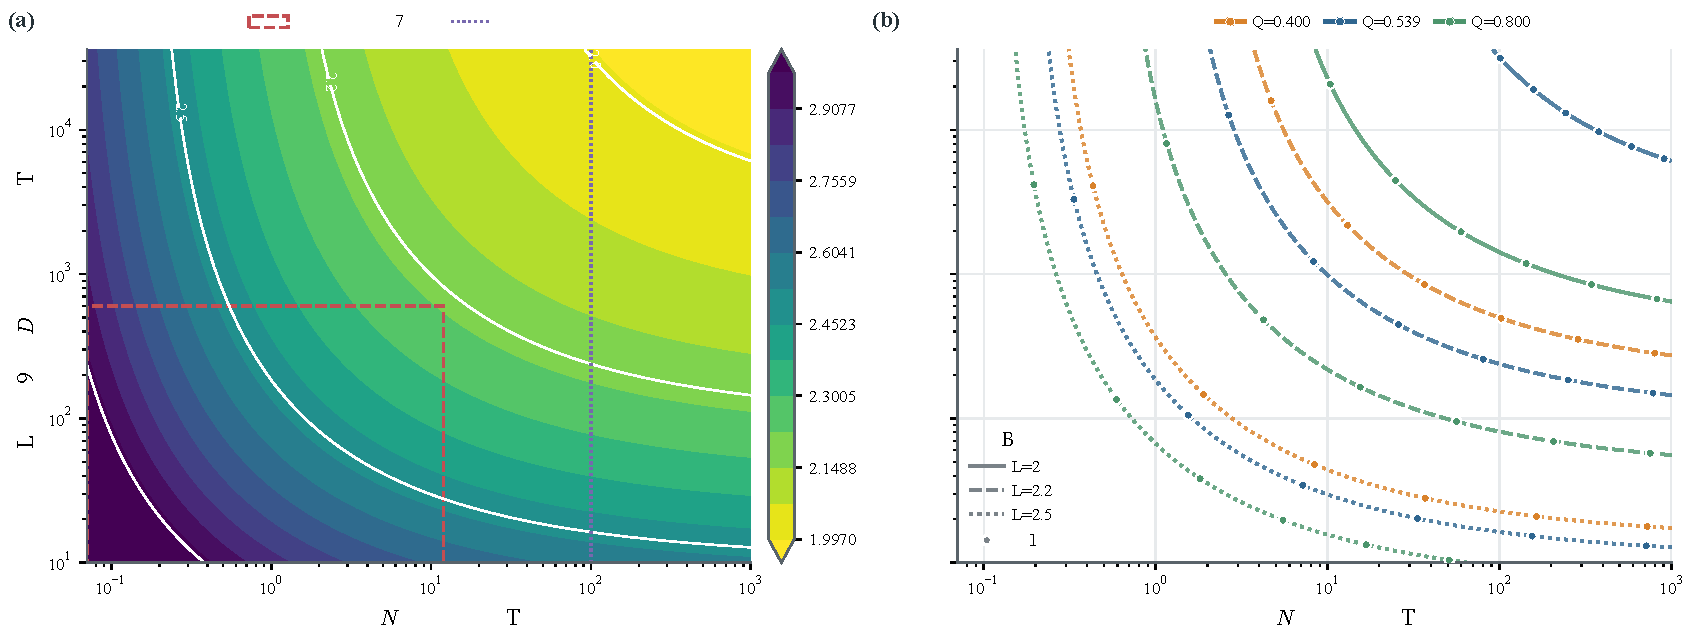
\includegraphics[width=\linewidth]{images/no2/P2R_F06_广义标度律地形与等损失前沿.pdf}
\caption{广义标度律的 Loss 地形（a）与不同质量下的等 Loss 前沿（b）}
\label{fig:p2_land}
\end{figure}

\subsection{边际效用、弹性与替代条件}

\subsubsection{边际效用与弹性}

对式~\eqref{eq:p2_GSL}（取 $\boldsymbol p=\boldsymbol p_{\mathrm{ref}}$、$s_Q=1$、未触及截断），各资源的边际效用为
\begin{equation}
-\frac{\partial L}{\partial N}=\frac{\alpha A n^{-\alpha}}{N},\qquad
-\frac{\partial L}{\partial D}=\frac{\beta B d^{-\beta}}{D},\qquad
-\frac{\partial L}{\partial Q}=c_Q\nu_Q(1-Q)^{\nu_Q-1},\qquad
\frac{\partial L}{\partial R}=\theta\,(L-E).
\label{eq:p2_marginal}
\end{equation}
为消除量纲，定义 Loss 弹性 $\epsilon_x=-\partial\ln L/\partial\ln x$：
\begin{equation}
\epsilon_N=\frac{\alpha An^{-\alpha}}{L},\qquad
\epsilon_D=\frac{\beta Bd^{-\beta}}{L},\qquad
\epsilon_Q=\frac{c_Q\nu_Q Q(1-Q)^{\nu_Q-1}}{L}.
\label{eq:p2_elasticity}
\end{equation}
在参考点，$\epsilon_N=0.048$、$\epsilon_D=0.034$、$\epsilon_Q=0.077$：\textbf{质量提高 1\% 对 Loss 的改善，相当于参数量提高 1.6\% 或数据量提高 2.3\%}。由式~\eqref{eq:p2_elasticity}，$\epsilon_N,\epsilon_D$ 随规模扩大按幂律衰减，而 $\epsilon_Q$ 的分子与规模无关——\textbf{规模越大，质量的相对重要性越高}。图~\ref{fig:p2_elas}(a) 显示，在 $D=150\mathrm{B}$ 下质量弹性在 $N\approx0.24\mathrm{B}$ 处超过参数弹性；在 27 个 $N$--$D$--$Q$ 网格状态上，质量弹性在总弹性中的平均份额为 $46.0\%$，有 16 个状态由质量主导（$s_Q=0.5$ 与 $1.5$ 时分别为 $30.8\%$、$55.5\%$）。

\begin{figure}[htbp]
\centering
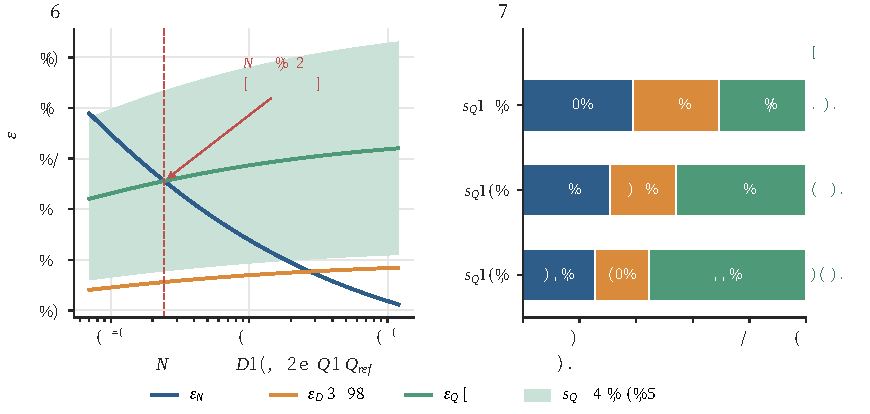
\includegraphics[width=\linewidth]{images/no2/P2R_F07_资源弹性组成状态图.pdf}
\caption{资源弹性随参数规模的变化（a）与不同质量映射强度下的弹性构成（b）}
\label{fig:p2_elas}
\end{figure}

\subsubsection{质量与规模的替代条件}

题目要求推导“质量提升 $\Delta Q$ 等价于参数增加多少”的可计算条件。固定其余变量，令质量提升带来的 Loss 降幅为
\begin{equation}
\delta_Q(\Delta Q)=c_Q\left[(1-Q)^{\nu_Q}-(1-Q-\Delta Q)^{\nu_Q}\right]e^{\theta R(\boldsymbol p)} .
\label{eq:p2_deltaQ}
\end{equation}

\begin{theorem}[质量—规模替代条件]\label{thm:subst}
在广义标度律~\eqref{eq:p2_GSL} 下，存在有限的参数量增幅 $r_N$，使
\[L\big(N(1+r_N),D,Q\big)=L(N,D,Q+\Delta Q)\]
成立的充要条件是
\begin{equation}
\delta_Q(\Delta Q)<A\,n^{-\alpha}e^{\theta R(\boldsymbol p)},
\label{eq:p2_cond_N}
\end{equation}
即质量提升带来的收益小于参数项的全部剩余可降低量。此时等价增幅有闭式解
\begin{equation}
r_N=\left[1-\frac{\delta_Q}{An^{-\alpha}e^{\theta R}}\right]^{-1/\alpha}-1,\qquad
r_D=\left[1-\frac{\delta_Q}{Bd^{-\beta}e^{\theta R}}\right]^{-1/\beta}-1,
\label{eq:p2_rN}
\end{equation}
其中 $r_D$ 的存在条件为 $\delta_Q<Bd^{-\beta}e^{\theta R}$。
\end{theorem}

\noindent\textbf{证明。}等价方程为 $An^{-\alpha}\left[1-(1+r_N)^{-\alpha}\right]e^{\theta R}=\delta_Q$。左端关于 $r_N\in(0,\infty)$ 连续严格递增，取值范围为 $\left(0,An^{-\alpha}e^{\theta R}\right)$，故有解当且仅当式~\eqref{eq:p2_cond_N} 成立，解出即得式~\eqref{eq:p2_rN}。$r_D$ 同理。\hfill$\square$

\textbf{数值结果。}在参考点（$N=1\mathrm{B}$、$D=150\mathrm{B}$、$Q=0.539$、$\boldsymbol p=\boldsymbol p_{\mathrm{ref}}$）取 $\Delta Q=0.1$，得 $\delta_Q=0.0362$，代入式~\eqref{eq:p2_rN}：
\begin{equation}
r_N=37.3\%,\qquad r_D=56.9\%,
\end{equation}
即\textbf{质量提高 0.1 的 Loss 改善，等价于参数量增加 37.3\% 或训练数据量增加 56.9\%}（图~\ref{fig:p2_equiv}(a)），与数值求根结果完全一致。

\textbf{替代的临界规模。}条件~\eqref{eq:p2_cond_N} 的右端随 $n$ 递减。令其等于 $\delta_Q$，得到临界规模
\begin{equation}
n_c=\left(\frac{A}{\delta_Q}\right)^{1/\alpha},\qquad d_c=\left(\frac{B}{\delta_Q}\right)^{1/\beta}.
\label{eq:p2_critical}
\end{equation}
对 $\Delta Q=0.1$，$N_c\approx820\mathrm{B}$、$D_c\approx3.1\times10^{14}$ Token。当模型参数超过约 8200 亿，或训练数据超过约 300 万亿 Token（已超过公开可用人类文本总量的估计\cite{villalobos2024rundata}）时，\textbf{再多的参数或数据也无法弥补 0.1 的质量差距}，质量成为不可替代的资源。该结论属于远超观测范围的外推，应理解为趋势判断；但它从模型层面解释了“数据墙”下高质量数据的战略价值。

图~\ref{fig:p2_equiv}(b) 给出等价增幅对质量映射强度 $s_Q$ 与基线质量的敏感性：$s_Q=1.5$ 时等价增幅升至 $63.2\%$（参数）与 $101.4\%$（数据）；当基线质量已高（$Q=0.8$）且 $s_Q=1.5$ 时，质量提升触及上限 $Q=1$，等价增幅回落至 $24.9\%$ 与 $37.1\%$。

\begin{figure}[htbp]
\centering
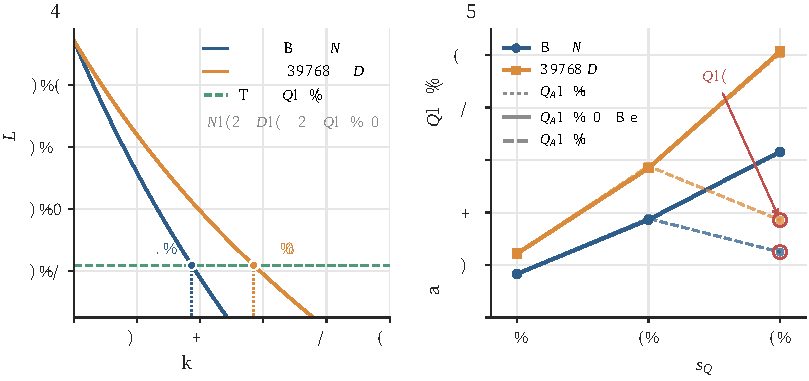
\includegraphics[width=\linewidth]{images/no2/P2R_F08_质量提升的有限资源等价量.pdf}
\caption{质量提升 $0.1$ 的等价资源增幅（a）及其对映射强度的敏感性（b）}
\label{fig:p2_equiv}
\end{figure}

注意，上述等价是“Loss 意义上的等价”，并未计入提升质量所需的算力。“同样多花一份算力，投向参数还是投向质量更划算”取决于单位算力的边际收益之比，这正是问题三 KKT 条件（式~\eqref{eq:p3_kkt}）所刻画的内容。

\subsubsection{领域之间的替代与互补}

由问题一 Scheff\'e 交互项的 bootstrap 结果（\S\ref{sec:problem1}），136 个领域对中有 75 对为稳定互补、没有稳定替代关系。结合广义标度律，可以给出领域 $i,j$ 间的\textbf{替代弹性}判据：在参考配比处，若 $\partial^2 R/\partial p_i\partial p_j<0$，则同时增加两个领域的份额比分别增加更有利（互补）；反之为替代。由于配比项以 $e^{\theta R}$ 乘在可约损失上，这种互补关系在所有规模上成比例保持，其绝对价值随可约损失的缩小而缩小。

\subsection{模型检验}

\subsubsection{外部验证}

冻结 B1 参数后，对 B2、B4、B5、B10 直接做预测（图~\ref{fig:p2_ext}）。跨模型族记录 B4 与文献数据 B5 的 Spearman 系数分别达 $0.983$ 与 $0.959$，说明\textbf{标度律对新模型族保持了正确的排序}；B4、B5 的 RMSE 为 $0.293$、$0.198$，绝对偏差主要来自不同模型族的分词器与验证集差异，体现为不可约项 $E$ 的平移。半合成族外轨迹 B2 的 RMSE 较大（$1.243$），Spearman 为 $0.788$，存在系统性的校准差。B10 为按标度律估算的 Loss（RMSE $0.001$），只作量级对照，不计为独立证据。

\begin{figure}[htbp]
\centering
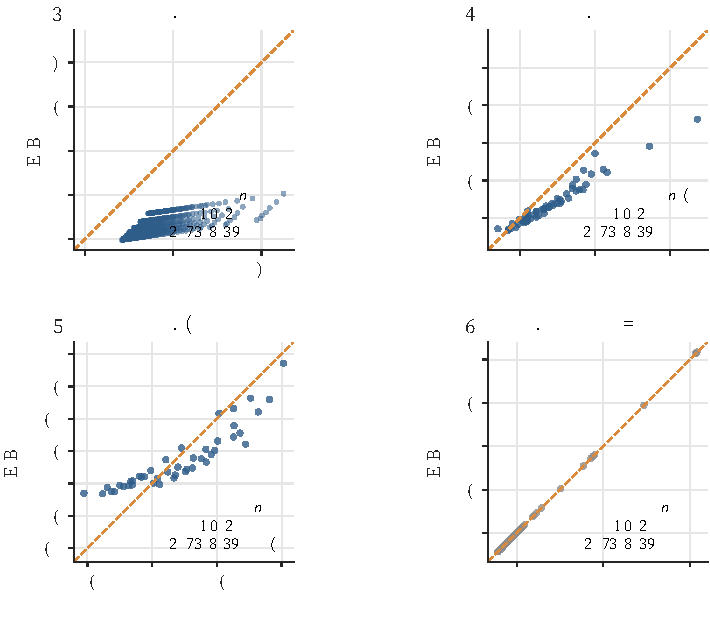
\includegraphics[width=0.92\linewidth]{images/no2/P2R_F10_经典标度律外部证据验证.pdf}
\caption{经典标度律在 B2、B4、B5、B10 上的外部验证}
\label{fig:p2_ext}
\end{figure}

\subsubsection{质量响应的压力测试}

B7 主网格中 Loss 随质量总体下降（中位数由 $Q=0.1$ 时的 $2.76$ 降至 $Q=1$ 时的 $2.39$），与 GQ2 方向一致；B6 为 B7 的子集，其质量响应与 B7 一致。半合成扩展网格 B8 则在大规模与远端外推区出现“质量越高 Loss 越高”的反向响应和 $L=0.5$ 截断地板，地板记录比例随参数规模增至 $38.3\%$（图~\ref{fig:p2_stress}）。这类响应违背基本常识，因此 B8 不参与模型选择，只用于标出外推风险区。

\begin{figure}[htbp]
\centering
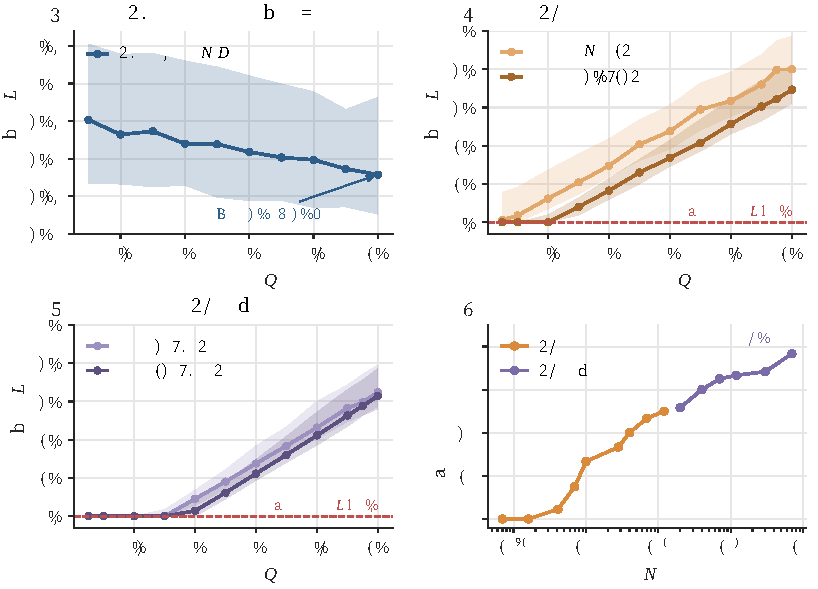
\includegraphics[width=\linewidth]{images/no2/P2R_F04_B7与B8质量响应压力测试.pdf}
\caption{B7 主质量网格与 B8 扩展网格的质量响应及截断地板比例}
\label{fig:p2_stress}
\end{figure}

\subsubsection{百亿参数以上的外推}

B1/B7 的观测支持域为 $N\in[0.07,12]\mathrm{B}$、$D\in[10,300]\mathrm{B}$。B9 给出百亿参数以上模型的规模信息，其规模已超出支持域 1--3 个数量级；B10 的 Loss 是按标度律估算的，与本文预测高度吻合（RMSE $0.001$），但只能说明二者使用了相近的外推公式，不能作为外推正确的证据。因此本文对超出支持域的预测统一标记为外推：参数—数据项的外推有 Chinchilla 系列研究的独立支持\cite{hoffmann2022compute,besiroglu2024chinchilla}，可信度较高；质量项与配比项的外推依赖假设~\ref{hyp:quality} 与假设~\ref{hyp:mix}，其中配比项的尺度不变性已在三个数量级上得到检验。

\subsection{问题二小结}

\begin{conclusionbox}
\textbf{问题二主要结论}
\begin{enumerate}
\item 提出同时包含 $N,D,Q,\boldsymbol p$ 的广义标度律 $L=E+\big[An^{-\alpha}+Bd^{-\beta}+c_Q(1-Q)^{\nu_Q}\big]e^{\theta R(\boldsymbol p)}$，在 $Q=1$、$\boldsymbol p=\boldsymbol p_{\mathrm{ref}}$ 时严格退化为经典形式，并保证 $L>E$。
\item 经典项的留一规模 RMSE 为 $1.47\times10^{-4}$，参数—数据可分性得到数据坍缩检验的支持；质量项选择加性惩罚 GQ2（成块验证 RMSE $0.072$，较 GQ1 降低 $38.7\%$），质量每提高 $0.1$ 使 Loss 降低约 $0.036$。
\item 配比效应的绝对强度随规模下降 $69\%$，但其相对可约损失的系数 $\theta\approx0.085$ 在 1M--1B 三个数量级上保持稳定，检验了“配比效应尺度不变”假设；近优配比可使可约损失降低约 $17.6\%$。
\item 质量提升 $0.1$ 等价于参数量增加 $37.3\%$ 或数据量增加 $56.9\%$；给出了替代存在的充要条件与临界规模闭式解：当 $N\gtrsim820\mathrm{B}$ 或 $D\gtrsim3\times10^{14}$ Token 时，质量差距无法再由规模弥补。领域之间以互补关系为主。
\end{enumerate}
\end{conclusionbox}
